%!TEX encoding = UTF-8 Unicode
% -*- coding: UTF-8; -*-
% vim: set fenc-utf-8

\chapter{Diagrammes de séquence de conception}
\label{s:sequence_conception}

Ce chapitre présente les diagrammes de séquence de conception associée aux fonctionnalitées de l'application.

\section{Convertir les coordonnées de la souris en coordonnées réelles}
\label{sec:convertir_coordonnees_souris}

%\begin{figure}[htpb]
%    \centering
%    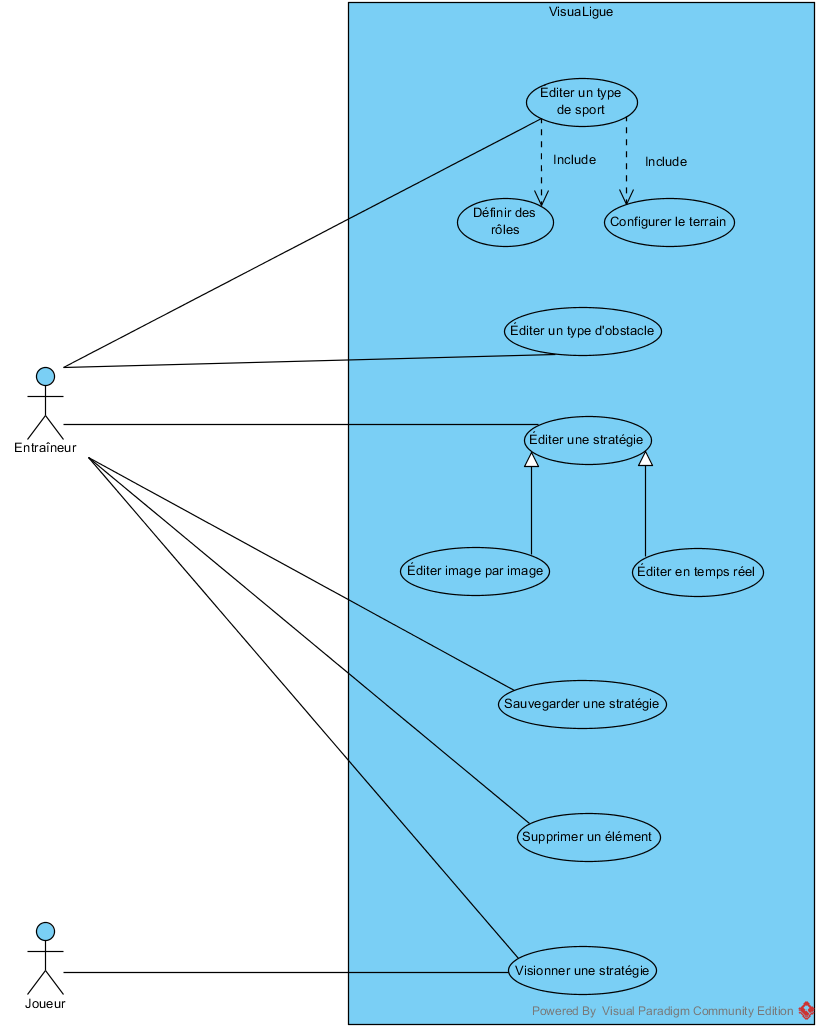
\includegraphics[scale=0.7]{fig/cas_utilisation_diag.png}
%    \caption{Diagramme de séquence de conception pour Convertir les coordonnées de la souris en coordonnées réelles}
%    \label{fig:dsc_pixel_en_reel}
%\end{figure}


\section{Ajouter un joueur}
\label{sec:ajouter_joueur}

\section{Convertir un clic de souris en la sélection d'un objet de jeu}
\label{convertir_clic_en_objet}

\section{Édition en mode image par image}
\label{sec:edition_image_par_image}

\section{Édition en mode temps réel}
\label{sec:edition_temps_reel}

\section{Visionner le jeu}
\label{sec:visionner_jeu}